% !TEX TS-program = pdflatex
\documentclass[11pt]{article}

% -------------------- Packages --------------------
\usepackage[a4paper,margin=1in]{geometry}
\usepackage{amsmath,amssymb}
\usepackage[T1]{fontenc}
\usepackage{lmodern}
\usepackage{xcolor}
\usepackage{tcolorbox}
\tcbuselibrary{skins,breakable}
\usepackage{enumitem}
\usepackage{hyperref}
\usepackage{tikz}
\usetikzlibrary{arrows.meta,positioning}

\pagestyle{empty}

% -------------------- Dark Theme Colors --------------------
\definecolor{bg}{HTML}{000000}
\definecolor{pairbg}{HTML}{121212}
\definecolor{solbg}{HTML}{0A0A0A}
\definecolor{border}{HTML}{2A2A2A}
\definecolor{text}{HTML}{FFFFFF}
\definecolor{muted}{HTML}{C9CDD3}
\definecolor{gold}{HTML}{FFD700}
\definecolor{green}{HTML}{4ADE80}
\definecolor{cyan}{HTML}{38BDF8}

\pagecolor{bg}
\color{text}

\hypersetup{
  colorlinks=true,
  linkcolor=cyan,
  urlcolor=cyan
}

\setlength{\parindent}{0pt}
\setlength{\parskip}{10pt}

\setlist[itemize]{left=1.4em,itemsep=6pt,topsep=6pt}
\setlist[enumerate]{left=1.6em,itemsep=4pt,topsep=4pt}

% -------------------- tcolorbox Base --------------------
\tcbset{
  enhanced,
  breakable,
  arc=12pt,
  boxrule=0.8pt,
  left=16pt,right=16pt,top=12pt,bottom=12pt
}

\newtcolorbox{QAPair}[1]{%
  colback=pairbg,
  colbacklower=solbg,
  colframe=border,
  coltext=text,
  title=\textcolor{gold}{\bfseries #1},
  fonttitle=\bfseries,
  coltitle=text,
  segmentation style={draw=border, dashed, line width=0.6pt},
}

\newtcolorbox{QuickBox}{%
  colback=pairbg,
  colframe=cyan,
  coltext=text,
  fontupper=\color{text},
  borderline north={4pt}{0pt}{cyan},
  arc=14pt,
  boxrule=0.8pt
}

% Helper for step headings
\newcommand{\Step}[1]{\textcolor{muted}{\textbf{Step #1:}}}

% Small helper for relation tables
\newcommand{\RelTableHeader}[2]{%
\begin{center}
\renewcommand{\arraystretch}{1.2}
\setlength{\tabcolsep}{10pt}
\begin{tabular}{c|#2}
\hline
#1\\ \hline
}

\newcommand{\RelTableFooter}{%
\hline
\end{tabular}
\end{center}
}

% TikZ styles for arrow diagrams
\tikzset{
  nodebox/.style={draw=border, rounded corners=8pt, inner sep=6pt, text=text, fill=solbg},
  arr/.style={-Latex, line width=0.8pt, draw=cyan}
}

% ============================================================
\begin{document}

\begin{center}
{\LARGE\bfseries \textcolor{gold}{Exercise 3.4 --- Solutions}}\\[-2pt]
\end{center}

\begin{QuickBox}
{\color{cyan}\bfseries Quick formulas (Binary Relations)}\par\medskip
\begin{itemize}
\item A \textbf{binary relation} from $A$ to $B$ is any subset of $A\times B$.
\item \textbf{Number of relations:} $\#\text{relations}=2^{|A\times B|}=2^{|A|\cdot |B|}$.
\item \textbf{On a set $A$:} relations on $A$ are subsets of $A\times A$, so $\#=2^{|A|^2}$.
\item \textbf{Domain:} $\operatorname{Dom}(R)=\{x:\exists y,(x,y)\in R\}$,\quad
\textbf{Range:} $\operatorname{Ran}(R)=\{y:\exists x,(x,y)\in R\}$.
\item \textbf{Inverse relation:} $R^{-1}=\{(y,x):(x,y)\in R\}$.
\end{itemize}
\end{QuickBox}

% ============================================================
% Q1
\begin{QAPair}{Question 1}
\textcolor{gold}{\bfseries Question:} Find the number of binary relations in the following cases:\\
(i) $A=\{1,3\},\ B=\{0,2,4\}$ \quad
(ii) $n(C)=7$ \quad
(iii) $D=\{1,3,5\}$.\\
\tcblower
\textcolor{green}{\bfseries Answer (step-wise):}
\[
\begin{aligned}
\Step{1}\;& \#\text{relations from }A\text{ to }B \;=\; 2^{|A\times B|}=2^{|A|\cdot|B|}.\\
\Step{2}\;& (i)\ |A|=2,\ |B|=3 \Rightarrow |A\times B|=2\cdot 3=6 \Rightarrow \#=2^6=64.\\[3pt]
\Step{3}\;& (ii)\ \text{Relations on }C \text{ (i.e., }C\to C):\ \#=2^{|C\times C|}=2^{7^2}=2^{49}.\\[3pt]
\Step{4}\;& (iii)\ \text{Relations on }D:\ |D|=3 \Rightarrow \#=2^{3^2}=2^9=512.
\end{aligned}
\]
\end{QAPair}

% ============================================================
% Q2
\begin{QAPair}{Question 2}
\textcolor{gold}{\bfseries Question:} Find \textbf{all possible} binary relations in each case and mention the number in each case:\\
(i) $A=\{\sqrt2,\sqrt3,\sqrt5\},\ B=\{\sqrt[3]{5}\}$\\
(ii) $C=\{\pi,e\}$\\
(iii) $D=\{5\},\ E=\{1,10\}$.\\
\tcblower

\textcolor{green}{\bfseries (i) Relations from $A$ to $B$}\par
Let $b=\sqrt[3]{5}$. Then
\[
A\times B=\{(\sqrt2,b),(\sqrt3,b),(\sqrt5,b)\}.
\]
\[
\Step{1}\; |A\times B|=3 \Rightarrow \#=2^3=8.
\]
All 8 relations (all subsets of $A\times B$):
\[
\begin{aligned}
R_0&=\varnothing\\
R_1&=\{(\sqrt2,b)\},\quad
R_2=\{(\sqrt3,b)\},\quad
R_3=\{(\sqrt5,b)\}\\
R_4&=\{(\sqrt2,b),(\sqrt3,b)\},\quad
R_5=\{(\sqrt2,b),(\sqrt5,b)\},\quad
R_6=\{(\sqrt3,b),(\sqrt5,b)\}\\
R_7&=\{(\sqrt2,b),(\sqrt3,b),(\sqrt5,b)\}.
\end{aligned}
\]

\textcolor{green}{\bfseries (ii) Relations on $C$}\par
\[
C\times C=\{(\pi,\pi),(\pi,e),(e,\pi),(e,e)\}.
\]
\[
\Step{1}\; |C\times C|=4 \Rightarrow \#=2^4=16.
\]
All 16 relations:
\[
\begin{aligned}
R_0&=\varnothing\\
R_1&=\{(\pi,\pi)\},\ R_2=\{(\pi,e)\},\ R_3=\{(e,\pi)\},\ R_4=\{(e,e)\}\\
R_5&=\{(\pi,\pi),(\pi,e)\},\ 
R_6=\{(\pi,\pi),(e,\pi)\},\ 
R_7=\{(\pi,\pi),(e,e)\}\\
R_8&=\{(\pi,e),(e,\pi)\},\ 
R_9=\{(\pi,e),(e,e)\},\ 
R_{10}=\{(e,\pi),(e,e)\}\\
R_{11}&=\{(\pi,\pi),(\pi,e),(e,\pi)\},\ 
R_{12}=\{(\pi,\pi),(\pi,e),(e,e)\}\\
R_{13}&=\{(\pi,\pi),(e,\pi),(e,e)\},\ 
R_{14}=\{(\pi,e),(e,\pi),(e,e)\}\\
R_{15}&=\{(\pi,\pi),(\pi,e),(e,\pi),(e,e)\}=C\times C.
\end{aligned}
\]

\textcolor{green}{\bfseries (iii) Relations from $D$ to $E$}\par
\[
D\times E=\{(5,1),(5,10)\},\qquad |D\times E|=2 \Rightarrow \#=2^2=4.
\]
All 4 relations:
\[
\varnothing,\quad \{(5,1)\},\quad \{(5,10)\},\quad \{(5,1),(5,10)\}.
\]
\end{QAPair}

% ============================================================
% Q3
\begin{QAPair}{Question 3}
\textcolor{gold}{\bfseries Question:} If $P=\{7,8,9\}$, find two binary relations from $P$ to $P$. Also find domain and range of each relation.\\
\tcblower
\textcolor{green}{\bfseries Answer (step-wise):}

\textcolor{green}{\bfseries Relation 1 (Identity relation)}\par
\[
R_1=\{(7,7),(8,8),(9,9)\}.
\]
\[
\begin{aligned}
\Step{1}\;& \operatorname{Dom}(R_1)=\{7,8,9\}\quad (\text{all first elements})\\
\Step{2}\;& \operatorname{Ran}(R_1)=\{7,8,9\}\quad (\text{all second elements})
\end{aligned}
\]

\textcolor{green}{\bfseries Relation 2 (``less than'' inside $P$)}\par
\[
R_2=\{(7,8),(7,9),(8,9)\}.
\]
\[
\begin{aligned}
\Step{1}\;& \operatorname{Dom}(R_2)=\{7,8\}.\\
\Step{2}\;& \operatorname{Ran}(R_2)=\{8,9\}.
\end{aligned}
\]
\end{QAPair}

% ============================================================
% Q4
\begin{QAPair}{Question 4}
\textcolor{gold}{\bfseries Question:} Let $H=\{5,6,7,8,9\}$ and $G=\{5,7,9,11\}$. Write the following relations from $H$ to $G$ in \textbf{tabular form}:\\
(i) is equal to \quad (ii) is less than \quad (iii) is greater than \quad
(iv) is one less than \quad (v) is one greater than \quad (vi) is two less than.\\
\tcblower

\textcolor{green}{\bfseries Convention:} Put \textbf{1} if $(h,g)$ is in the relation, otherwise \textbf{0}.\\

% (i)
\textcolor{green}{\bfseries (i) ``is equal to'' ($h=g$)}\par
\begin{center}
\renewcommand{\arraystretch}{1.2}
\setlength{\tabcolsep}{8pt}
\begin{tabular}{c|cccc}
$H\backslash G$ & $5$ & $7$ & $9$ & $11$\\ \hline
$5$ & 1 & 0 & 0 & 0\\
$6$ & 0 & 0 & 0 & 0\\
$7$ & 0 & 1 & 0 & 0\\
$8$ & 0 & 0 & 0 & 0\\
$9$ & 0 & 0 & 1 & 0\\ \hline
\end{tabular}
\end{center}

% (ii)
\textcolor{green}{\bfseries (ii) ``is less than'' ($h<g$)}\par
\begin{center}
\renewcommand{\arraystretch}{1.2}
\setlength{\tabcolsep}{8pt}
\begin{tabular}{c|cccc}
$H\backslash G$ & $5$ & $7$ & $9$ & $11$\\ \hline
$5$ & 0 & 1 & 1 & 1\\
$6$ & 0 & 1 & 1 & 1\\
$7$ & 0 & 0 & 1 & 1\\
$8$ & 0 & 0 & 1 & 1\\
$9$ & 0 & 0 & 0 & 1\\ \hline
\end{tabular}
\end{center}

% (iii)
\textcolor{green}{\bfseries (iii) ``is greater than'' ($h>g$)}\par
\begin{center}
\renewcommand{\arraystretch}{1.2}
\setlength{\tabcolsep}{8pt}
\begin{tabular}{c|cccc}
$H\backslash G$ & $5$ & $7$ & $9$ & $11$\\ \hline
$5$ & 0 & 0 & 0 & 0\\
$6$ & 1 & 0 & 0 & 0\\
$7$ & 1 & 0 & 0 & 0\\
$8$ & 1 & 1 & 0 & 0\\
$9$ & 1 & 1 & 0 & 0\\ \hline
\end{tabular}
\end{center}

% (iv)
\textcolor{green}{\bfseries (iv) ``is one less than'' ($h=g-1$ i.e., $g=h+1$)}\par
\begin{center}
\renewcommand{\arraystretch}{1.2}
\setlength{\tabcolsep}{8pt}
\begin{tabular}{c|cccc}
$H\backslash G$ & $5$ & $7$ & $9$ & $11$\\ \hline
$5$ & 0 & 0 & 0 & 0\\
$6$ & 0 & 1 & 0 & 0\\
$7$ & 0 & 0 & 0 & 0\\
$8$ & 0 & 0 & 1 & 0\\
$9$ & 0 & 0 & 0 & 0\\ \hline
\end{tabular}
\end{center}

% (v)
\textcolor{green}{\bfseries (v) ``is one greater than'' ($h=g+1$ i.e., $g=h-1$)}\par
\begin{center}
\renewcommand{\arraystretch}{1.2}
\setlength{\tabcolsep}{8pt}
\begin{tabular}{c|cccc}
$H\backslash G$ & $5$ & $7$ & $9$ & $11$\\ \hline
$5$ & 0 & 0 & 0 & 0\\
$6$ & 1 & 0 & 0 & 0\\
$7$ & 0 & 0 & 0 & 0\\
$8$ & 0 & 1 & 0 & 0\\
$9$ & 0 & 0 & 0 & 0\\ \hline
\end{tabular}
\end{center}

% (vi)
\textcolor{green}{\bfseries (vi) ``is two less than'' ($h=g-2$ i.e., $g=h+2$)}\par
\begin{center}
\renewcommand{\arraystretch}{1.2}
\setlength{\tabcolsep}{8pt}
\begin{tabular}{c|cccc}
$H\backslash G$ & $5$ & $7$ & $9$ & $11$\\ \hline
$5$ & 0 & 1 & 0 & 0\\
$6$ & 0 & 0 & 0 & 0\\
$7$ & 0 & 0 & 1 & 0\\
$8$ & 0 & 0 & 0 & 0\\
$9$ & 0 & 0 & 0 & 1\\ \hline
\end{tabular}
\end{center}
\end{QAPair}

% ============================================================
% Q5
\begin{QAPair}{Question 5}
\textcolor{gold}{\bfseries Question:} Let $C=\{2,4,6\}$, $D=\{4,6,8,9,12\}$ and
\[
R=\{(x,y)\mid x\in C,\ y\in D \ \wedge\ x \text{ is a factor of } y\}.
\]
(i) Write $R$ in tabular form.\;
(ii) Find domain and range of $R$.\;
(iii) Find $R^{-1}$.\;
(iv) Represent $R$ by arrow diagram.\\
\tcblower

\textcolor{green}{\bfseries Step-wise construction of $R$:}
\[
\begin{aligned}
\Step{1}\;& x=2 \text{ divides } 4,6,8,12 \Rightarrow (2,4),(2,6),(2,8),(2,12).\\
\Step{2}\;& x=4 \text{ divides } 4,8,12 \Rightarrow (4,4),(4,8),(4,12).\\
\Step{3}\;& x=6 \text{ divides } 6,12 \Rightarrow (6,6),(6,12).
\end{aligned}
\]
So
\[
R=\{(2,4),(2,6),(2,8),(2,12),(4,4),(4,8),(4,12),(6,6),(6,12)\}.
\]

\textcolor{green}{\bfseries (i) Tabular form}\par
\begin{center}
\renewcommand{\arraystretch}{1.2}
\setlength{\tabcolsep}{8pt}
\begin{tabular}{c|ccccc}
$C\backslash D$ & $4$ & $6$ & $8$ & $9$ & $12$\\ \hline
$2$ & 1 & 1 & 1 & 0 & 1\\
$4$ & 1 & 0 & 1 & 0 & 1\\
$6$ & 0 & 1 & 0 & 0 & 1\\ \hline
\end{tabular}
\end{center}

\textcolor{green}{\bfseries (ii) Domain and range}\par
\[
\begin{aligned}
\Step{1}\;& \operatorname{Dom}(R)=\{2,4,6\} \quad (\text{all first components appear}).\\
\Step{2}\;& \operatorname{Ran}(R)=\{4,6,8,12\} \quad (\text{the second components used}).
\end{aligned}
\]

\textcolor{green}{\bfseries (iii) Inverse relation $R^{-1}$}\par
\[
\begin{aligned}
R^{-1}=\{&(4,2),(6,2),(8,2),(12,2),\\
&(4,4),(8,4),(12,4),\\
&(6,6),(12,6)\}.
\end{aligned}
\]

\textcolor{green}{\bfseries (iv) Arrow diagram of $R$}\par\medskip
\begin{center}
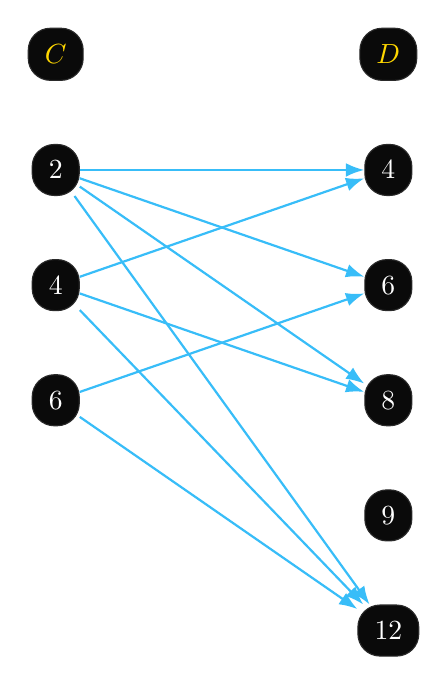
\begin{tikzpicture}[node distance=10mm and 25mm]
  \node[nodebox] (cTitle) {\textcolor{gold}{\bfseries $C$}};
  \node[nodebox, right=35mm of cTitle] (dTitle) {\textcolor{gold}{\bfseries $D$}};

  \node[nodebox, below=8mm of cTitle] (c2) {$2$};
  \node[nodebox, below=8mm of c2]     (c4) {$4$};
  \node[nodebox, below=8mm of c4]     (c6) {$6$};

  \node[nodebox, below=8mm of dTitle] (d4) {$4$};
  \node[nodebox, below=8mm of d4]     (d6) {$6$};
  \node[nodebox, below=8mm of d6]     (d8) {$8$};
  \node[nodebox, below=8mm of d8]     (d9) {$9$};
  \node[nodebox, below=8mm of d9]     (d12){$12$};

  % arrows from 2
  \draw[arr] (c2) -- (d4);
  \draw[arr] (c2) -- (d6);
  \draw[arr] (c2) -- (d8);
  \draw[arr] (c2) -- (d12);

  % arrows from 4
  \draw[arr] (c4) -- (d4);
  \draw[arr] (c4) -- (d8);
  \draw[arr] (c4) -- (d12);

  % arrows from 6
  \draw[arr] (c6) -- (d6);
  \draw[arr] (c6) -- (d12);
\end{tikzpicture}
\end{center}
\end{QAPair}

% ============================================================
% Q6
\begin{QAPair}{Question 6}
\textcolor{gold}{\bfseries Question:} Let
\[
R=\{(2,0),(4,2),(6,4),(8,6),(10,8)\}.
\]
(i) Write $R$ in set-builder form.\;
(ii) Find domain and range.\;
(iii) Write $R^{-1}$ in tabular and set-builder form.\;
(iv) Represent $R$ and $R^{-1}$ by arrow diagram.\\
\tcblower

\textcolor{green}{\bfseries (i) Set-builder form (step-wise):}
\[
\begin{aligned}
\Step{1}\;& \text{Notice that in every pair, } y=x-2.\\
\Step{2}\;& \text{The first elements are even numbers }2,4,6,8,10.\\
\Step{3}\;& R=\{(x,y)\mid x\in\{2,4,6,8,10\},\ y=x-2\}.
\end{aligned}
\]

\textcolor{green}{\bfseries (ii) Domain and range:}
\[
\operatorname{Dom}(R)=\{2,4,6,8,10\},\qquad
\operatorname{Ran}(R)=\{0,2,4,6,8\}.
\]

\textcolor{green}{\bfseries (iii) Inverse relation}
\[
R^{-1}=\{(0,2),(2,4),(4,6),(6,8),(8,10)\}.
\]
Set-builder form:
\[
\begin{aligned}
\Step{1}\;& \text{Swap coordinates: }(x,y)\in R \Rightarrow (y,x)\in R^{-1}.\\
\Step{2}\;& R^{-1}=\{(y,x)\mid x\in\{2,4,6,8,10\},\ y=x-2\}.
\end{aligned}
\]

\textcolor{green}{\bfseries Tabular form of $R$ (rows $A=\{2,4,6,8,10\}$, columns $B=\{0,2,4,6,8\}$)}\par
\begin{center}
\renewcommand{\arraystretch}{1.2}
\setlength{\tabcolsep}{8pt}
\begin{tabular}{c|ccccc}
$A\backslash B$ & $0$ & $2$ & $4$ & $6$ & $8$\\ \hline
$2$  & 1 & 0 & 0 & 0 & 0\\
$4$  & 0 & 1 & 0 & 0 & 0\\
$6$  & 0 & 0 & 1 & 0 & 0\\
$8$  & 0 & 0 & 0 & 1 & 0\\
$10$ & 0 & 0 & 0 & 0 & 1\\ \hline
\end{tabular}
\end{center}

\textcolor{green}{\bfseries Tabular form of $R^{-1}$ (rows $B$, columns $A$)}\par
\begin{center}
\renewcommand{\arraystretch}{1.2}
\setlength{\tabcolsep}{8pt}
\begin{tabular}{c|ccccc}
$B\backslash A$ & $2$ & $4$ & $6$ & $8$ & $10$\\ \hline
$0$ & 1 & 0 & 0 & 0 & 0\\
$2$ & 0 & 1 & 0 & 0 & 0\\
$4$ & 0 & 0 & 1 & 0 & 0\\
$6$ & 0 & 0 & 0 & 1 & 0\\
$8$ & 0 & 0 & 0 & 0 & 1\\ \hline
\end{tabular}
\end{center}

\textcolor{green}{\bfseries (iv) Arrow diagrams}\par\medskip
\begin{center}
\begin{minipage}{0.48\linewidth}
\centering
\textcolor{muted}{\bfseries $R$}\par\smallskip
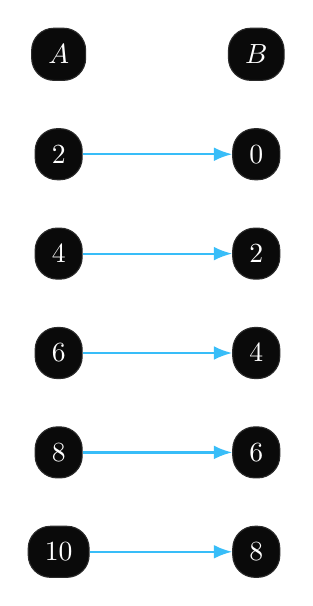
\begin{tikzpicture}[node distance=7mm and 16mm]
  \node[nodebox] (Ltitle) {$A$};
  \node[nodebox, right=18mm of Ltitle] (Rtitle) {$B$};

  \node[nodebox, below=6mm of Ltitle] (a2) {$2$};
  \node[nodebox, below=6mm of a2] (a4) {$4$};
  \node[nodebox, below=6mm of a4] (a6) {$6$};
  \node[nodebox, below=6mm of a6] (a8) {$8$};
  \node[nodebox, below=6mm of a8] (a10){$10$};

  \node[nodebox, below=6mm of Rtitle] (b0) {$0$};
  \node[nodebox, below=6mm of b0] (b2) {$2$};
  \node[nodebox, below=6mm of b2] (b4) {$4$};
  \node[nodebox, below=6mm of b4] (b6) {$6$};
  \node[nodebox, below=6mm of b6] (b8) {$8$};

  \draw[arr] (a2) -- (b0);
  \draw[arr] (a4) -- (b2);
  \draw[arr] (a6) -- (b4);
  \draw[arr] (a8) -- (b6);
  \draw[arr] (a10)-- (b8);
\end{tikzpicture}
\end{minipage}\hfill
\begin{minipage}{0.48\linewidth}
\centering
\textcolor{muted}{\bfseries $R^{-1}$}\par\smallskip
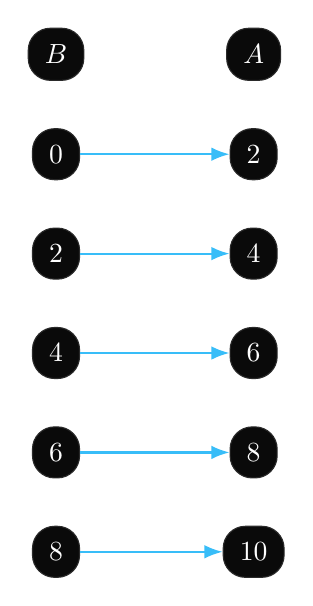
\begin{tikzpicture}[node distance=7mm and 16mm]
  \node[nodebox] (Ltitle) {$B$};
  \node[nodebox, right=18mm of Ltitle] (Rtitle) {$A$};

  \node[nodebox, below=6mm of Ltitle] (b0) {$0$};
  \node[nodebox, below=6mm of b0] (b2) {$2$};
  \node[nodebox, below=6mm of b2] (b4) {$4$};
  \node[nodebox, below=6mm of b4] (b6) {$6$};
  \node[nodebox, below=6mm of b6] (b8) {$8$};

  \node[nodebox, below=6mm of Rtitle] (a2) {$2$};
  \node[nodebox, below=6mm of a2] (a4) {$4$};
  \node[nodebox, below=6mm of a4] (a6) {$6$};
  \node[nodebox, below=6mm of a6] (a8) {$8$};
  \node[nodebox, below=6mm of a8] (a10){$10$};

  \draw[arr] (b0) -- (a2);
  \draw[arr] (b2) -- (a4);
  \draw[arr] (b4) -- (a6);
  \draw[arr] (b6) -- (a8);
  \draw[arr] (b8) -- (a10);
\end{tikzpicture}
\end{minipage}
\end{center}
\end{QAPair}

% ============================================================
% Q7
\begin{QAPair}{Question 7}
\textcolor{gold}{\bfseries Question:} Let $A=\{0,1,3\}$ and $B=\{1,2,3,5,7\}$. Write
\[
R=\{(x,y)\mid x\in A,\ y\in B,\ \wedge\ y=2x+1\}
\]
in tabular form. Also find $R^{-1}$.\\
\tcblower

\textcolor{green}{\bfseries Step-wise:}
\[
\begin{aligned}
\Step{1}\;& x=0 \Rightarrow y=2(0)+1=1 \in B \Rightarrow (0,1)\in R.\\
\Step{2}\;& x=1 \Rightarrow y=3 \in B \Rightarrow (1,3)\in R.\\
\Step{3}\;& x=3 \Rightarrow y=7 \in B \Rightarrow (3,7)\in R.
\end{aligned}
\]
So
\[
R=\{(0,1),(1,3),(3,7)\}.
\]

\textcolor{green}{\bfseries Tabular form}\par
\begin{center}
\renewcommand{\arraystretch}{1.2}
\setlength{\tabcolsep}{8pt}
\begin{tabular}{c|ccccc}
$A\backslash B$ & $1$ & $2$ & $3$ & $5$ & $7$\\ \hline
$0$ & 1 & 0 & 0 & 0 & 0\\
$1$ & 0 & 0 & 1 & 0 & 0\\
$3$ & 0 & 0 & 0 & 0 & 1\\ \hline
\end{tabular}
\end{center}

\textcolor{green}{\bfseries Inverse relation:}
\[
R^{-1}=\{(1,0),(3,1),(7,3)\}.
\]
\end{QAPair}

% ============================================================
% Q8
\begin{QAPair}{Question 8}
\textcolor{gold}{\bfseries Question:} If $S=\{1,2,4,8\}$ and $T=\{3^0,3^1,3^2\}$, then write the following binary relations in tabular form.\\
\tcblower

\textcolor{green}{\bfseries First simplify $T$:}
\[
T=\{3^0,3^1,3^2\}=\{1,3,9\}.
\]
We will write the tabular forms for:
\[
\begin{aligned}
R_1&=\{(x,y)\mid x\in S,\ y\in T,\ x=y\}\\
R_2&=\{(x,y)\mid x\in S,\ y\in T,\ y<x\}\\
R_3&=\{(x,y)\mid x\in S,\ y\in T,\ x+y\in E\}\ \ (\text{$E=$ even integers})\\
R_4&=\{(x,y)\mid x\in S,\ y\in T,\ xy\in O\}\ \ (\text{$O=$ odd integers})\\
R_5&=\{(x,y)\mid x\in S,\ y\in T,\ y>2x\}.
\end{aligned}
\]

\textcolor{green}{\bfseries Column order: $T=\{1,3,9\}$, row order: $S=\{1,2,4,8\}$.}\par\medskip

\textcolor{green}{\bfseries (i) Tabular form of $R_1$ ($x=y$)}\par
\begin{center}
\renewcommand{\arraystretch}{1.2}
\setlength{\tabcolsep}{10pt}
\begin{tabular}{c|ccc}
$S\backslash T$ & $1$ & $3$ & $9$\\ \hline
$1$ & 1 & 0 & 0\\
$2$ & 0 & 0 & 0\\
$4$ & 0 & 0 & 0\\
$8$ & 0 & 0 & 0\\ \hline
\end{tabular}
\end{center}

\textcolor{green}{\bfseries (ii) Tabular form of $R_2$ ($y<x$)}\par
\begin{center}
\renewcommand{\arraystretch}{1.2}
\setlength{\tabcolsep}{10pt}
\begin{tabular}{c|ccc}
$S\backslash T$ & $1$ & $3$ & $9$\\ \hline
$1$ & 0 & 0 & 0\\
$2$ & 1 & 0 & 0\\
$4$ & 1 & 1 & 0\\
$8$ & 1 & 1 & 0\\ \hline
\end{tabular}
\end{center}

\textcolor{green}{\bfseries (iii) Tabular form of $R_3$ ($x+y$ even)}\par
(\textit{Since $1,3,9$ are odd, $x+y$ is even only when $x$ is odd $\Rightarrow x=1$.})\par
\begin{center}
\renewcommand{\arraystretch}{1.2}
\setlength{\tabcolsep}{10pt}
\begin{tabular}{c|ccc}
$S\backslash T$ & $1$ & $3$ & $9$\\ \hline
$1$ & 1 & 1 & 1\\
$2$ & 0 & 0 & 0\\
$4$ & 0 & 0 & 0\\
$8$ & 0 & 0 & 0\\ \hline
\end{tabular}
\end{center}

\textcolor{green}{\bfseries (iv) Tabular form of $R_4$ ($xy$ odd)}\par
(\textit{Product is odd only if both are odd. $y$ is always odd, so $x$ must be odd $\Rightarrow x=1$.})\par
\begin{center}
\renewcommand{\arraystretch}{1.2}
\setlength{\tabcolsep}{10pt}
\begin{tabular}{c|ccc}
$S\backslash T$ & $1$ & $3$ & $9$\\ \hline
$1$ & 1 & 1 & 1\\
$2$ & 0 & 0 & 0\\
$4$ & 0 & 0 & 0\\
$8$ & 0 & 0 & 0\\ \hline
\end{tabular}
\end{center}

\textcolor{green}{\bfseries (v) Tabular form of $R_5$ ($y>2x$)}\par
\begin{center}
\renewcommand{\arraystretch}{1.2}
\setlength{\tabcolsep}{10pt}
\begin{tabular}{c|ccc}
$S\backslash T$ & $1$ & $3$ & $9$\\ \hline
$1$ & 0 & 1 & 1\\
$2$ & 0 & 0 & 1\\
$4$ & 0 & 0 & 1\\
$8$ & 0 & 0 & 0\\ \hline
\end{tabular}
\end{center}
\end{QAPair}

% ============================================================
% Q9
\begin{QAPair}{Question 9}
\textcolor{gold}{\bfseries Question:} Find the domain and range in each case (using $S=\{1,2,4,8\}$ and $T=\{1,3,9\}$):\\
(i) $R_1=\{(x,y)\mid x\in S,\ y\in T,\ x=y\}$\\
(ii) $R_2=\{(x,y)\mid x\in S,\ y\in T,\ y<x\}$\\
(iii) $R_3=\{(x,y)\mid x\in S,\ y\in T,\ x+y\in E\}$\\
(iv) $R_4=\{(x,y)\mid x\in S,\ y\in T,\ xy\in O\}$\\
(v) $R_5=\{(x,y)\mid x\in S,\ y\in T,\ y>2x\}$.\\
\tcblower

\textcolor{green}{\bfseries (i) For $R_1$}
\[
\begin{aligned}
\Step{1}\;& R_1=\{(1,1)\}.\\
\Step{2}\;& \operatorname{Dom}(R_1)=\{1\},\quad \operatorname{Ran}(R_1)=\{1\}.
\end{aligned}
\]

\textcolor{green}{\bfseries (ii) For $R_2$}
\[
\begin{aligned}
\Step{1}\;& R_2=\{(2,1),(4,1),(4,3),(8,1),(8,3)\}.\\
\Step{2}\;& \operatorname{Dom}(R_2)=\{2,4,8\},\quad \operatorname{Ran}(R_2)=\{1,3\}.
\end{aligned}
\]

\textcolor{green}{\bfseries (iii) For $R_3$}
\[
\begin{aligned}
\Step{1}\;& \text{$x+y$ even only when }x=1 \Rightarrow R_3=\{(1,1),(1,3),(1,9)\}.\\
\Step{2}\;& \operatorname{Dom}(R_3)=\{1\},\quad \operatorname{Ran}(R_3)=\{1,3,9\}.
\end{aligned}
\]

\textcolor{green}{\bfseries (iv) For $R_4$}
\[
\begin{aligned}
\Step{1}\;& xy \text{ odd only when }x=1 \Rightarrow R_4=\{(1,1),(1,3),(1,9)\}.\\
\Step{2}\;& \operatorname{Dom}(R_4)=\{1\},\quad \operatorname{Ran}(R_4)=\{1,3,9\}.
\end{aligned}
\]

\textcolor{green}{\bfseries (v) For $R_5$}
\[
\begin{aligned}
\Step{1}\;& R_5=\{(1,3),(1,9),(2,9),(4,9)\}.\\
\Step{2}\;& \operatorname{Dom}(R_5)=\{1,2,4\},\quad \operatorname{Ran}(R_5)=\{3,9\}.
\end{aligned}
\]
\end{QAPair}

\end{document}
